\capitulo{4}{Técnicas y herramientas}

\section{Metodologías}

\subsection{Scrum}
La metodología Scrum~\cite{Scrum} es un marco de trabajo que es comúnmente usado para la gestión del desarrollo de un proyecto software y permite realizar entregas incrementales de valor en vez de realizar una única entrega en un periodo mayor de tiempo. Este marco de trabajo se fundamenta en separar los proyectos en entregas más pequeñas llamadas \textit{sprints}. En el caso de los \textit{sprints}, no existe una duración estándar, si no que al iniciar el proyecto, se decide esa duración. Para este proyecto los \textit{sprints} han sido de 2 semanas de manera general, y de manera excepcional 3 semanas.

Todo sprint se inicia realizando una planificación de las tareas del proyecto que se van a realizar durante su duración y, al terminar el sprint, se realiza una nueva reunión para revisar el estado de las tareas previstas para el sprint y una retrospectiva que permite detectar ineficiencias y errores para su posterior solución y mejora en el rendimiento del proyecto.

\subsection{Kanban}

Kanban~\cite{Kanban} es un sistema de apoyo visual cuyo objetivo es mejorar la eficiencia de los procesos a realizar mediante una gestión rápida del estado de las tareas. Esta metodología originaria de la marca de vehículos Toyota \footnote{Enlace a la \href{https://soka.gitlab.io/blog/post/2019-07-02-01-trello-origen-kanban-toyota-jit/}{ historia de kanban en Toyota}} consiste en una tabla visual en la que aparecen distintas columnas, siendo cada una de ellas un estado decidido por el equipo y no hay un estándar fijo. Comúnmente son las siguientes:
\begin{itemize}
    \item Pendiente de realizar
    \item En progreso
    \item Completado
\end{itemize}

Dentro de cada una de las columnas se encuentran todas las tareas pertenecientes al sprint actual, repartidas según su estado establecido por el equipo.

Una gran ventaja de este sistema es que permite al equipo de trabajo ver dónde se encuentran los cuellos de botella de las tareas ya que se van acumulando en esa columna. Al visualizar esto, se pueden tomar medidas rápidas para evitar así una pérdida de eficiencia.

Por otra parte, otra gran ventaja de esta metodología es su facilidad de uso ya que el flujo de acciones a realizar para la mantenibilidad del tablero es escaso.
\begin{enumerate}
    \item Se abre una nueva incidencia o desarrollo en el sprint, por lo que se coloca la tarea en la columna por hacer.
    \item Cuando el responsable de realizar esta tarea comienza a desarrollar la solución al problema propuesto, la tarea se pasa a la columna En Progreso.
    \item Una vez el desarrollador de la tarea termine, la pasa a la columna completado, indicando así al equipo que no es necesario invertir más tiempo y recursos a ese elemento.
\end{enumerate}


\subsubsection{Scrum y Kanban en Github}

Para poder aplicar estas metodologías a este proyecto, se han utilizado diferentes herramientas gratuitas de Github, las cuales nos permiten simular los \textit{sprints} y tener una batería de tareas que podemos gestionar en un tablero visual. 

\begin{enumerate}
    \item \textbf{Tareas y \textit{sprints}:}
    Las tareas de este proyecto se han generado en el apartado de Issues de Github. Este apartado nos permite establecer un título y una descripción, así como realizar diferentes asignaciones tales como la persona encargada de resolverla, en que proyecto se encuentra, y en que \textit{milestone} ha de agruparse.

    Los \textit{milestones} mencionadas en la figura \ref{Milestones con Issues incluidas} son una herramienta que nos brinda Github y que nos permite simular los \textit{Sprints}. Dentro de esta herramienta se establece un título y descripción de lo que se va a tratar, así como una fecha de fin en la cual se asocian las tareas a realizar. Es importante destacar que uno de los puntos donde se diferencia una \textit{milestone} de un sprint es en la posibilidad de modificar la fecha de fin si es necesario, opción que en un sprint no se puede realizar.
    \begin{figure}[htbp]
        \centering
        \includegraphics[width=0.8\linewidth]{Imagenes/milestone.png}
        \caption{\textit{milestone} con Issues incluidas}
        \label{Milestones con Issues incluidas}
    \end{figure}
    \FloatBarrier

    \item \textbf{Projects:}
    Los proyectos de Github son una representación kanban de las tareas que se crean para poder llevar una visión rápida de las tareas. En este caso, estas dos herramientas son muy similares exceptuando pequeños matices, como el límite de trabajo en progreso, el cual en Github se puede gestionar de manera manual pero no es tan estricto como Kanban. En la figura \ref{Tablero de Github} se puede observar el tablero de Github utilizado durante este proyecto.
    \begin{figure}[htbp]
        \centering
        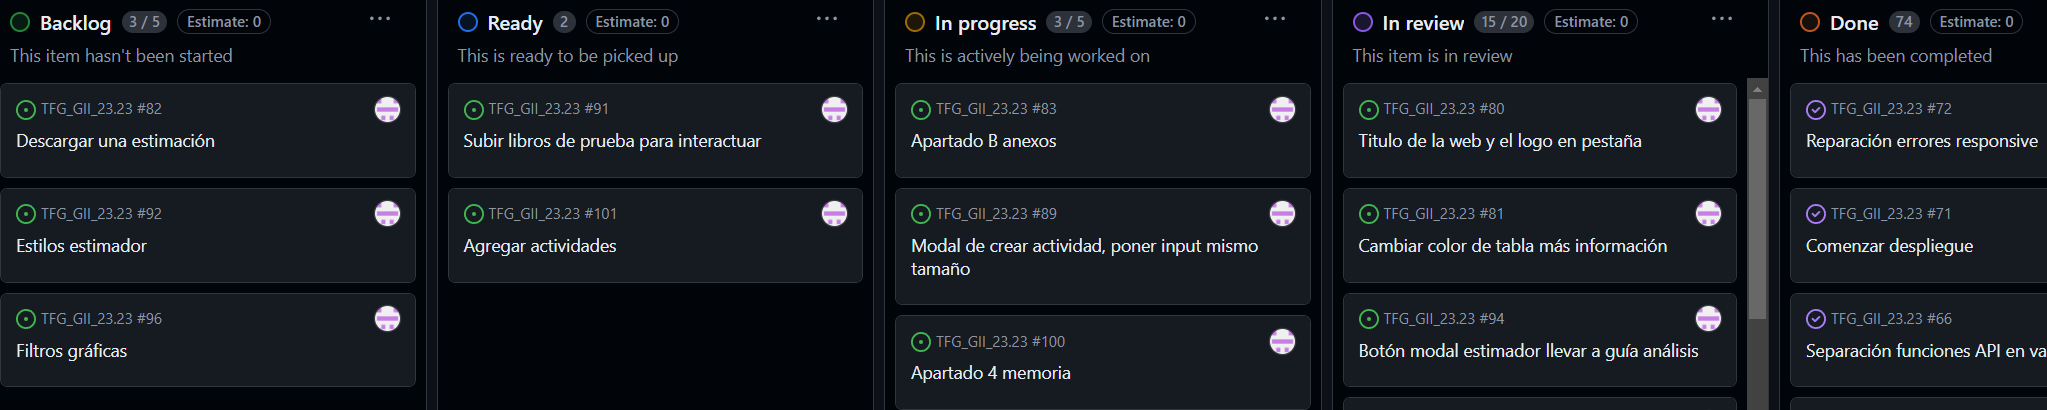
\includegraphics[width=0.8\linewidth]{Imagenes/TableroGithub.png}
        \caption{Tablero de Github}
        \label{Tablero de Github}
    \end{figure}
    \FloatBarrier
\end{enumerate}

\section{Frameworks utilizado para el desarrollo del proyecto}

\subsection{Herramienta \textit{Backend}: Flask}

Flask~\cite{Flask} es un microframework para Python que ha sido diseñado para facilitar el desarrollo de aplicaciones web. A diferencia de otros frameworks más complejos y rígidos, Flask proporciona la flexibilidad necesaria para adaptar la estructura del proyecto a las necesidades específicas de este. Ofrece un conjunto de herramientas que simplifican procesos como el enrutamiento, la gestión de sesiones y la integración con bases de datos. Inicialmente en el desarrollo del proyecto se ha utilizado esta herramienta tanto para el \textit{backend} como para el \textit{frontend}, sin embargo, se presentó la oportunidad de cambiar el sistema cuando ya se encontraba muy avanzado y migrar el \textit{frontend} a Angular y dejar este framework para la parte de \textit{backend}. Esto ocurrió debido a la toma de contacto con esta nueva tecnología en mis prácticas curriculares y la posibilidad de desarrollar elementos más complejos gracias a este \textit{framework}.

\subsubsection{Funcionalidades y Ventajas de Flask}

La elección de Flask se debe a su capacidad para manejar tanto aspectos básicos como avanzados del desarrollo web:

\begin{itemize}
    \item \textbf{Desarrollo Ágil:} Flask permite un rápido desarrollo y prototipado, lo que es ideal para los ciclos de iteración del TFG.
    \item \textbf{Simplicidad y Flexibilidad:} Su simplicidad  facilita la comprensión del código, lo que es fundamental para un TFG, donde la claridad y la documentación son clave.
    \item \textbf{Ecosistema Completo:} Existe una amplia variedad de extensiones disponibles que permiten añadir funcionalidades adicionales según sea necesario, sin sobrecargar el núcleo de la aplicación.
    \item \textbf{Licencia:} Flask está disponible bajo la licencia BSD, una licencia de software libre que permite la reutilización y distribución del código con pocas restricciones.
\end{itemize}

 \subsubsection{Bibliotecas utilizadas:}

 \begin{itemize}
     \item Flask y sus derivados:
     Estas bibliotecas de Flask son las básicas para tener la importación completa del framework y poder utilizar todas sus funcionalidades. 
     \item \href{https://beautiful-soup-4.readthedocs.io/en/latest/}{beautifulSoup4}: 
     Es una librería que se encarga de permitir obtener información de un archivo HTML, así como métodos para realizar búsquedas o modificaciones en ese archivo. En este proyecto se utiliza para obtener los datos de un libro durante la búsqueda automática de libros.
     \item \href{https://pypi.org/project/bcrypt/}{bcrypt}:
     Proporciona funciones para la gestión de contraseñas, como el cifrado y la verificación de una contraseña. Esto es realmente útil ya que no va a ser nunca necesario descifrar una contraseña para poder comparar si es la correcta o no.
     \item \href{https://gunicorn.org/}{gunicorn}: Es un servidor WSGI que permite a Flask manejar llamadas de manera concurrente y así permitir la simultaneidad.
     \item \href{https://openpyxl.readthedocs.io/en/stable/}{openpyxl}:
     Esta librería permite crear y leer archivos excel, lo cual es bastante util para que los administrasdores puedan gestionar diferentes aspectos de la web.
     \item \href{https://requests.readthedocs.io/en/latest/}{requests}:
     Esta librería permite realizar llamadas de distintos tipos a una web remota. Esta librería se utiliza durante el web scraping 
     \item \href{https://www.sqlalchemy.org/}{SQLAlchemy}: Permite tener una interfaz de alto nivel para poder tratar con los datos de una base de datos relacional, donde se encuentran recogidos todos los datos de la aplicación web.
 \end{itemize}

\subsection{Herramienta \textit{Frontend}: Angular}
 Angular~\cite{Angular} es un framework de desarrollo de aplicaciones web creado y mantenido por Google.
 Este framework está especialmente diseñado para poder crear webs robustas y muy rápidas y para este proyecto se ha usado en la parte \textit{frontend} después de la decisión de refactorizar desde Flask.

 
 \subsubsection{Características y ventajas de Angular}

 \begin{itemize}
     \item Estilo de la aplicación y arquitectura: 

     Angular tiene un concepto de SPA (Single Page Application) y una arquitectura basada en componentes. Esto nos permite mantener una modularidad absoluta de los elementos de la web y poder reutilizarlos siempre que se quiera. Además, la ventaja principal de un SPA es que todos los elementos, si no se encuentra activo el Lazy Loading, se cargan en una misma página, pero se ocultan y se muestran en base a la redirección necesaria, por lo que los tiempos son mucho menores entre el cambio de páginas.

     \item Lenguaje utilizado en este framework:
     
     Angular utiliza TypeScript para su programación lógica y para la parte visible al usuario se utiliza HTML y CSS. Typescript es un superconjunto de JavaScript que permite tener más características y funcionalidades que si se utilizase únicamente JavaScript

     \item Inyección de dependencias:
    Una gran ventaja de Angular es la facilidad para realizar inyecciones de dependencias en componentes y servicios para poder interconectarse de una manera rápida, evitar posible código duplicado y poder mantener una organización clara y simple que puede fomentar la eficiencia en el desarrollo
     
 \end{itemize}

 \subsubsection{Bibliotecas utilizadas:}
 \begin{itemize}
     \item PrimeNG~\cite{PrimeNG}/PrimeIcons~\cite{PrimeIcons}:
     Es una librería de componentes de interfaz de usuario que proporciona un amplio catálogo de componentes personalizables, como tablas, formularios, menús y gráficos mientras que PrimeIcons es un conjunto de iconos utilizados con PrimeNG para mejorar la apariencia de la aplicación.

  
     \item SweetAlerts2~\cite{SweetAlert2}: Es una librería  para crear alertas personalizables en aplicaciones web. Permite mostrar alertas con diferentes estilos, iconos y botones, mejorando la experiencia de usuario y la sencillez de la mantenibilidad.
 \end{itemize}
 


\section{Desarrolllo de prototipo Web}
\subsection{Justinmind}

Justinmind~\cite{Justinmind} es una herramienta de prototipado interactiva utilizada en este proyecto para diseñar la interfaz de la web de libros de la prehistoria. Fue elegida por su facilidad de uso, y amplia biblioteca de widgets.

\paragraph{Ventajas de Justinmind}

\begin{itemize}
    \item Interactividad: Simulación realista de la interfaz final de usuario
    \item Versatilidad: Adecuada para prototipos de baja y alta fidelidad.
\end{itemize}


Justinmind ha sido fundamental para definir y validar la experiencia del usuario de manera inicial, realizar pruebas de usabilidad y facilitar la comunicación del diseño entre los desarrolladores y el cliente.

 \section{Hosting de los archivos}
 \subsection{GitHub (Repositorio)}
 GitHub~\cite{Github} es una plataforma que utiliza el sistema de control de versiones Git para almacenar y permitir gestionar los proyectos creados de software de manera colaborativa. Además contiene una serie de herramientas muy variadas para comprobar el estado actual de las tareas relacionadas con el proyecto. Estas herramientas son las mencionadas anteriormente en el apartado de Kanban y Scrum.

 \subsubsection{Ventajas de la utilización de Github}
 \begin{itemize}
     \item \textbf{Sistema de versionado:} 
     Esta herramienta permite mantener un sistema de versiones y poder consultar que cambios se han realizado y el momento en el que se han realizado. Esto es de especial relevancia en caso de que una nueva versión genere errores o incompatibilidades, ya que podemos revertir los cambios y restaurar a una versión anterior.
     \item \textbf{Existencia de Issues: }
     Tal como se ha expuesto antes, esta herramienta permite la gestión de tareas a través de las Issues, lo cual nos permite indicar y ver de manera rápida los desarrollos o incidencias existentes sin necesidad de utilizar ninguna herramienta de terceros.
     \item \textbf{Sistema colaborativo: }
     Al permitir un sistema colaborativo a tiempo real, Github da la oportunidad a que varios integrantes del equipo puedan realizar modificaciones y poder ser más eficientes en términos temporales. En el caso del desarrollo de este proyecto, esta opción de colaboración se ha utilizado para la creación de incidencias durante la fase de despliegue.
 \end{itemize}
 
 \subsection{Render (\textit{Backend})}
 Render~\cite{Render} es una plataforma de servicios que se ha utilizado para desplegar la parte de la aplicación escrita en Python, consistente en la API que contiene toda la lógica de la aplicación web. Esta decisión se ha tomado principalmente por el bajo costo del despliegue en las condiciones necesarias, la sencillez y la compatibilidad con el lenguaje generado.
 
 Además de eso, la balanza se ha decantado por esta herramienta por los siguientes motivos:
 \begin{itemize}
     \item \textbf{Despliegue automático: }
     Esta herramienta permite tener una conexión activa con el repositorio de Github y al detectar un nuevo cambio en el repositorio, automáticamente lanza un nuevo despliegue para que el servidor siempre se encuentre en la última versión disponible.
     \item \textbf{Configuración del despliegue simple: }
     Al utilizar la herramienta incorporada de crear la API es necesario rellenar campos de configuración para establecer el lugar de los archivos y como se lanza cada uno de los necesarios. A diferencia de otros servicios, Render facilita todo este trabajo con formularios muy simples incluyendo un ejemplo e información muy completa relativo a cada campo.
     Además de ese formulario, de una manera rápida y sencilla se pueden modificar las variables de entorno necesarias para el correcto funcionamiento de la aplicación.
     \item \textbf{Existencia de discos de guardado de datos: }
     Tal como se menciona en el título del apartado, Render permite tener a disposición del proyecto un disco para poder guardar los datos deseados. En este proyecto se ha utilizado para poder gestionar los datos recogidos en la base de datos que usa el API.
     La gran ventaja de esto es que cada 24 horas se realiza una copia de seguridad que se puede restablecer en caso de necesidad.
 \end{itemize}
 
 \subsection{Netlify (\textit{Frontend})}
 Netlify~\cite{Netlify}, al igual que Render, es una plataforma de alojamiento para proyectos software, pero está especialmente orientada hacia el \textit{Frontend} y Angular, por lo que, al estar optimizada para este framework, en el caso de este proyecto se convierte en una opción muy interesante teniendo en cuenta que contiene una opción de despliegue gratuito. Para consolidar esta herramienta como la elegida para poder realizar este despliegue, se tuvieron en cuenta las siguientes ventajas:

 \begin{itemize}
     \item \textbf{Despliegue continuo: }
     Al igual que Render para el \textit{backend}, Netlify ofrece la posibilidad de tras realizar una conexión exitosa con la cuenta de Github donde se encuentra el repositorio, cargar y realizar las actualizaciones necesarias en el sistema de despliegue después de que se haya detectado un cambio en el repositorio.
     \item \textbf{Configuración simple: }
     Esta característica es importante ya que, aunque para Angular se necesiten hacer pasos adicionales ya que es un SPA y puedan aumentar la complejidad del despliegue, con unos pocos pasos se puede realizar la conexión inicial sin ningún problema. En el caso de que fallase algo, Netlify contiene una zona de Logs donde se puede observar todos los pasos que realiza durante el despliegue y nos puede dar indicaciones del problema que ha surgido.
    \item \textbf{Gestión de versiones: }
    Existe un apartado dentro de Netlify que permite volver a un despliegue anterior en caso de que se produzcan errores o incompatibilidades con la versión más reciente. Como gran punto a favor, es importante mencionar que, a diferencia de Render, mientras se realiza un nuevo despliegue, este se realiza en segundo plano, manteniendo así la disponibilidad de la web el máximo tiempo posible.
 \end{itemize}

\section{Herramientas para la escritura de la memoria}

\subsection{Overleaf}
Overleaf~\cite{Overleaf} es una plataforma diseñada para redactar documentos en \LaTeX. Overleaf es una herramienta pensada principalmente para investigadores ya que permite colaboración en tiempo real y una organización de páginas mucho más limpia que otras herramientas.

A continuación se muestran algunas ventajas por las que se usa este editor de texto.
\begin{itemize}
    \item \textbf{Compilación automática: }
    A diferencia de otras herramientas que trabajan con \LaTeX, Overleaf permite compilar en tiempo real el documento para ir llevando una depuración de fallos mientras se está redactando.
    \item \textbf{Historial de versiones: } Esta herramienta permite la posibilidad de poder revisar los cambios que se han ido realizando con el tiempo, al igual que ofrece Github para sus archivos. Esto es muy beneficioso ya que de esta manera podemos recuperar datos eliminados por error.
    \item \textbf{Acceso Online: }
    Overleaf al ser una plataforma web, permite acceder desde cualquier parte a los documentos guardados y así no tener que realizar transferencias de archivos a otros dispositivos, lo cual puede llegar a ser tedioso en el caso de que sea necesario en repetidas ocasiones.
    \item \textbf{Adaptación al usuario:} Cuenta con dos tipos de vista para poder redactar el documento, una vista de código, donde se puede aplicar código de programación \LaTeX y comandos directamente por el usuario, o la vista de editor, una vista mucho más simple para usuarios que no están familiarizados con el lenguaje.
\end{itemize}

\subsection{Draw.io}
Draw.io~\cite{Drawio} es una herramienta en línea con opción a descarga que permite realizar diagramas de diferentes tipos para mostrar de una manera gráfica procesos o un esquema un diagrama de flujo.
Dentro de las opciones disponibles en el mercado, esta herramienta tiene varias ventajas:
\begin{itemize}
    \item \textbf{Personalización: }
    Esta herramienta permite una gran personalización de todos los elementos que la componen, permitiendo así realizar los diagramas de la manera óptima y visual para el usuario final.
    \item \textbf{Exportación: }
    Para poder tener más libertad durante la manipulación de los diagramas, Drawio permite exportar en diferentes extensiones para poder generar el archivo más adecuado para el posterior uso de ese diagrama. En el caso de este proyecto se ha utilizado la exportación como PNG para poder incluir el archivo dentro de los Anexos.
    \item \textbf{Precio: } A diferencia de muchas herramientas, todos estos beneficios se pueden obtener de forma totalmente gratuita y sin necesidad de registros, por lo que es una buena opción para reducir gastos de desarrollo del proyecto.
\end{itemize}

\section{Otras herramientas usadas}

\subsection{Postman}
Postman~\cite{Postman} es una herramienta que permite realizar llamadas a APIs durante las fases de desarrollo y testing. A través de Postman se pueden realizar peticiones HTTP de diferentes tipos y mostrar los datos enviados por la API sin tener limitaciones de formato.
A continuación se muestran algunas de las ventajas clave de esta herramienta:
\begin{itemize}
    \item \textbf{Organización de carpetas:}
    Postman permite tener una organización de carpetas fijas con llamadas preestablecidas para que no sea necesario escribir de nuevo la petición entera, lo que es muy eficiente en términos temporales.
    \item \textbf{Múltiples tipos de solicitudes HTTP: } 
    Este servicio permite no solo realizar llamadas de obtención o envío de datos si no que permite realizar además llamadas de modificación de datos (PUT) y de borrado (DELETE). Esto da la oportunidad de usando un único programa poder comprobar si los desarrollos que se van realizando se completan satisfactoriamente, tanto en tiempo como el contenido resultante.
    \item \textbf{Interfaz y precio: }
    La interfaz de esta herramienta es muy sencilla y gráfica por lo que sin necesidad de una extensa documentación se puede comenzar a utilizar el programa. Además, el software es gratuito y no es necesario iniciar sesión, por lo que el proceso de instalación y puesta en marcha es muy sencillo.
\end{itemize}

\section{Análisis Comparativo entre Google Books API y Amazon Books API}
Debido a la necesidad de integrar una API de libros para poder realizar llamadas, se realiza una comparativa inicial entre Google Books API ~\cite{GoogleBooks} y Amazon Books API~\cite{AmazonBooks} para obtener el mejor candidato para implantar en el trabajo.
\subsection{Accesibilidad y Documentación}
\begin{itemize}
    \item \textbf{Google Books API:} Ofrece accesibilidad superior y documentación detallada. Proporciona una clave de API gratuita con un límite de 1,000 solicitudes diarias.
    \item \textbf{Amazon Books API:} Requiere afiliación a Amazon Advertising API y está orientada hacia usuarios con propósitos comerciales. La documentación es robusta pero más compleja.
\end{itemize}

\subsection{Amplitud de Datos Disponibles}
\begin{itemize}
    \item \textbf{Google Books API:} Acceso a más de 25 millones de libros con información extensa, ideal para proyectos educativos o bibliotecarios.
    \item \textbf{Amazon Books API:} Proporciona datos orientados a ventas y reseñas, incluyendo rankings y precios, útil para análisis de mercado, pero no tanto para nuestra intencionalidad.
\end{itemize}

\subsection{Facilidad de Integración y Uso}
\begin{itemize}
    \item \textbf{Google Books API:} Fácil integración gracias a su estructura basada en REST y compatibilidad con múltiples lenguajes de programación.
    \item \textbf{Amazon Books API:} Requiere comprensión avanzada de las API de Amazon y sus requisitos de autenticación, generando una curva de aprendizaje más grande.
\end{itemize}

\subsection{Restricciones de Uso y Limitaciones}
\begin{itemize}
    \item \textbf{Google Books API:} Tiene limitaciones en el número de solicitudes diarias, pero de manera general es aceptable para la escala de este proyecto.
    \item \textbf{Amazon Books API:} Limitaciones más estrictas en cuanto a la frecuencia de las solicitudes y acceso a algunos datos.
\end{itemize}

La elección de la API de Google Books se justifica por su accesibilidad, amplia gama de datos bibliográficos, facilidad de integración, y una cuota de solicitudes gratuitas mayor. Esto la hace ideal para este proyecto ya que nos brinda más facilidades y más datos que nos resulten relevantes.


\tablaSmall{Herramientas y tecnologías utilizadas en cada parte del proyecto}{l c c c c}{herramientasportipodeuso}
{\multicolumn{1}{l}{Herramientas} & App Angular & API REST & BD & Memoria \\}{ 
HTML5 & X & & &\\
CSS3 & X & & &\\
PrimeNG & X & & &\\
TypeScript & X & & &\\
AngularJS & X & & &\\
SweetAlert2 & X & & &\\
Netlify & X & & &\\
Python & & X & &\\
Flask framework & & X & &\\
BeautifulSoup4 & & X & &\\
Bcrypt & & X & &\\
Google Books API & & X & &\\
JSON & X & X & &\\
Gunicorn & & X & &\\
Openpyxl & & X & &\\
Requests & & X & &\\
Postman & & X & &\\
Render & & X & X &\\
SQLLite & & & X &\\
SQLAlchemy & & X & X &\\
Github & X & X & X & X\\
Overleaf & & & & X\\
Drawio & & & & X\\
Justinmind & & & & X\\
} 
